\documentclass[a4paper]{article}

\usepackage{fullpage} % Package to use full page
\usepackage{parskip} % Package to tweak paragraph skipping
\usepackage{tikz} % Package for drawing

\usepackage{hyperref}
\usepackage{amsmath}
\usepackage{amssymb}
\usepackage{amsthm}
\usepackage{enumitem}

\usepackage{subcaption}

\title{COMP 465 Assignment 4}
\author{Ling Tan}
\date{2018/11/13}

\begin{document}

\maketitle

\section{32.1-2} Suppose that all characters in the pattern $P$ are different. Show how to accelerate NAIVE-STRING-MATCHER to run in time $O(n)$ on an $n$-character text $T$.\\
\textcolor{blue}{Answer:}
Because all characters in the pattern $P$ are different, when $P[j]\neq T[i]$, we can shift $s+j$ instead of $s+1$.
\section{32.2-3}
Show how to extend the Rabin-Karp method to handle the problem of looking for a given $m\times m$ pattern in an $n \times n$ array of characters. (The pattern may be shifted vertically and horizontally, but it may not be rotated.)\\
\textcolor{blue}{Answer:} 
    \begin{enumerate}
        \item Calculate the column $[0\ldots 0, 0\ldots m-1]$ and the row $[0\ldots 0, m-1\ldots 0]$ using a hash function. But when shifting vertically or horizontally, using a rolling hash function $s$:
            \begin{align*}
                s[i, j+1..j+m] & = s[i, j\ldots j+m-1] - s[i, j] + s[i, j+m]\\
                s[i+1..i+m, j] & = s[i..i+m-1, j] - s[i,j ] + s[i+m, j]
            \end{align*}
        So, in total is $O((n-m+1)^2)$.
        \item Calculate the hash value of $P$, the costing time is $O(m^2)$.
        \item For every match, the comparison is $O(m^2)$.
    \end{enumerate}
\section{34.2-2}
Prove that if $G$ is an undirected bipartite graph with an odd number of vertices, then $G$ is nonhamiltonian.\\
\textcolor{blue}{Answer:} By contradiction.
\begin{proof}
Let $G=(V,E), V=\{v_1,v_2,\ldots, v_n\}$ is a bipartite graph with two disjoint vertices set $S$ and $T$ where there is no edge between vertices in the same set. Assume there is a Hamilton cycle $v_1, v_2, \cdots, v_n, v_1$. If $v_1\in S$, then $v_2\in T$ (and vice versa). Because $|E|$ is odd, we know that $v_n\in S$. Since $v_1\in S$, there is no edge between $v_n$ and $v_1$, this leads to a contradiction. Therefore, $G$ is not Hamiltonian.

\end{proof}

\section{34.2-7}
Show that the hamiltonian-path problem can be solved in polynomial time on directed acyclic graphs. Give an efficient algorithm for the problem.\\
\textcolor{blue}{Answer:}
    \begin{enumerate}
        \item Topological sorting the graph: $\Theta(V+E)$
        \item Check whether every vertex is adjacent to next one.
        \item If it is, then there is a Hamilton path.
        \item If not, then the un-adjacent vertex is not reachable since the graph is topological sorted, thus the graph has no Hamilton path.
    \end{enumerate}
\section{34.3-1}
Verify that the circuit in Figure 34.8(b) is unsatisfiable.\\
\textcolor{blue}{Answer:} Figure 34.8(b) is equivalent to
    \begin{equation*}
        l=(l_1\land l_2) \land (l_2\lor l_3) \land (l_3)
    \end{equation*}
    where
    \begin{align*}
        l_1 &= x_1\lor x_2\\
        l_2 &= \lnot(\lnot x_3)=x_3\\
        l_3 &= x_1\land x_2\land \lnot x_3
    \end{align*}
    \begin{center}
        \begin{tabular}{ccc|ccc|c}
             $x_1$ & $x_2$ & $x_3$ & $l_1$ & $l_2$ & $l_3$ & $l$\\
             \hline
             0 & 0 & 0 & 0 & 0 & 0 & 0\\
             0 & 0 & 1 & 0 & 1 & 0 & 0\\
             0 & 1 & 0 & 1 & 0 & 0 & 0\\
             0 & 1 & 1 & 1 & 1 & 0 & 0\\
             1 & 0 & 0 & 1 & 0 & 0 & 0\\
             1 & 0 & 1 & 1 & 1 & 0 & 0\\
             1 & 1 & 0 & 1 & 0 & 1 & 0\\
             1 & 1 & 1 & 1 & 1 & 0 & 0
        \end{tabular}
    \end{center}
    No output of $1$, thus it is unsatisfiable.

\section{34.5-6}
Show that the Hamiltonian-path problem is NP-complete.\\
\textcolor{blue}{Answer:}
\begin{enumerate}
    \item For a given solution $S$ to a graph $G$, we can verify whether the $S$ is a Hamilton path by just following the vertices in $S$ in polynomial computing time, so the Hamiltonian-path problem is in \textit{NP}.
    \item We need to show Hamilton cycle problem $\leq_p$ Hamilton path problem.\\
    Given an instance of Hamilton cycle problem on a graph $G=(V,E)$, we construct an instance of the Hamilton path problem on a graph $G'$ by the following rules:
    \begin{enumerate}
        \item Copy all the vertices and edges in $G$ to $G'$.
        \item Add a vertex $v_2$ to $G'$.
        \item Choose an arbitrary vertex $v_1$ in $G'$, connection $v_2$ to all the vertices that $v_1$ connected to.
        \item Add two vertices $v_1',v_2'$ to $G'$.
        \item Connect $v_1'$ to $v_1$, connect $v_2'$ to $v_2$.
    \end{enumerate}
    This construction can be done in polynomial time.\\
    If there is a Hamilton cycle in $G$, we know that cycle can leave from $v_1$ and return back to $v_1$. So we can construct a Hamilton path in $G'$ such that it starts from $v_1'$, then follow that same path of the Hamilton cycle in $G$, and then when it reaches that last vertex before $v_1$, it continue moves to $v_2$, and finally goes to $v_2'$.\\
    Conversely, if there is a Hamilton path in $G'$, saying the path starts from $v_1'$ and ends with $v_2'$, we can construct a Hamilton cycle by removing $v_1',v_2'$ and let $v_1=v_2$.\\
    Hamilton cycle problem is \textit{NP}-complete, thus Hamilton path problem is \textit{NP}-complete.
\end{enumerate}

\section{} The longest-simple-cycle problem is the problem of determining a simple cycle (no repeated vertices) of maximum length in a graph. Show that this problem is NP-complete.\\
\textcolor{blue}{Answer:} This is an optimization problem, the corresponding decision problem is: given a graph $G$ and an integer $k$, is there a simple cycle with length $\geq k$. Use $P_k$ to denote this decision problem.
\begin{enumerate}
    \item Given a solution $S$ of $P_k$ to a graph $G=(V,E)$, we can verify whether it is a simple cycle with the length $\geq k$ in polynomial computing time. So $P_k\in \textit{NP}$.
    \item We need to show $\text{Hamilton cycle problem}\leq_p P_k$.\\
    Given an instance of Hamilton cycle problem on a graph $G=(V,E)$, we can construct an instance of $P_k$ on a graph $G'$, where $G'$ is a copy of $G$. If there is a Hamilton cycle in $G$, then there is a simple cycle in $G'$ with the length of $k\geq|V|$, and vice versa.
\end{enumerate}

\section{} Professor Nixon proposes the following heuristic to solve the vertex-cover problem. Repeatedly select a vertex of highest degree, and remove all of its incident edges. Give an example to show that the professor's heuristic does not have an approximation ratio of $2$.
(Hint: Try a bipartite graph with vertices of uniform degree on the left and vertices of varying degree on the right.)\\
\textcolor{blue}{Answer:} Consider the bipartite graph:
\begin{center}
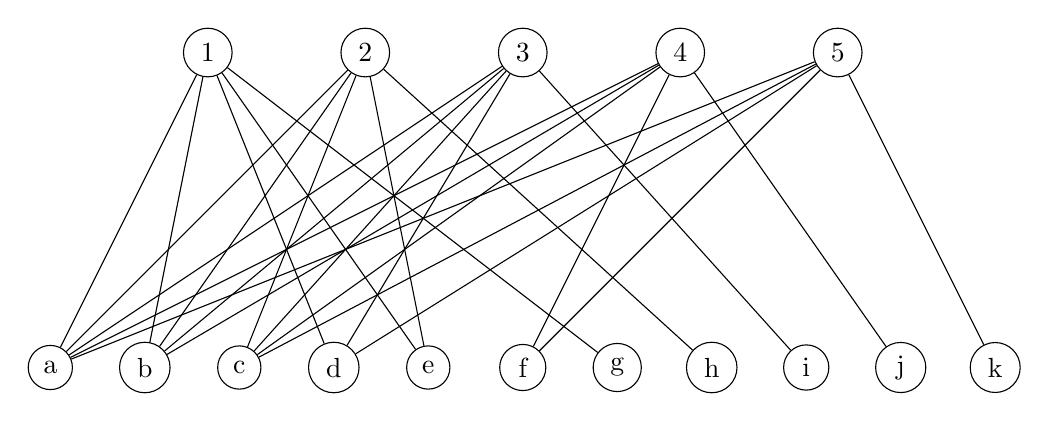
\begin{tikzpicture}[auto]
   \begin{scope}[every node/.style={circle,draw=black}]
    \node (l1) at (-4,1) {1};
    \node (l2) at (-2,1) {2};
    \node (l3) at (0,1) {3};
    \node (l4) at (2,1) {4};
    \node (l5) at (4,1) {5};
    \node (r1) at (-6,-3) {a};
    \node (r2) at (-4.8,-3) {b};
    \node (r3) at (-3.6,-3) {c};
    \node (r4) at (-2.4,-3) {d};
    \node (r5) at (-1.2,-3) {e};
    \node (r6) at (0,-3) {f};
    \node (r7) at (1.2,-3) {g};
    \node (r8) at (2.4,-3) {h};
    \node (r9) at (3.6,-3) {i};
    \node (r10) at (4.8,-3) {j};
    \node (r11) at (6,-3) {k};
   \end{scope}
   \begin{scope}[every edge/.style={draw=black}]
    \draw  (r1) edge node{ } (l1);
    \draw  (r1) edge node{ } (l2);
    \draw  (r1) edge node{ } (l3);
    \draw  (r1) edge node{ } (l4);
    \draw  (r1) edge node{ } (l5);
    \draw  (r2) edge node{ } (l1);
    \draw  (r2) edge node{ } (l2);
    \draw  (r2) edge node{ } (l3);
    \draw  (r2) edge node{ } (l4);
    \draw  (r3) edge node{ } (l2);
    \draw  (r3) edge node{ } (l3);
    \draw  (r3) edge node{ } (l4);
    \draw  (r3) edge node{ } (l5);
    \draw  (r4) edge node{ } (l1);
    \draw  (r4) edge node{ } (l3);
    \draw  (r4) edge node{ } (l5);
    \draw  (r5) edge node{ } (l1);
    \draw  (r5) edge node{ } (l2);
    \draw  (r6) edge node{ } (l4);
    \draw  (r6) edge node{ } (l5);
    \draw  (r7) edge node{ } (l1);
    \draw  (r8) edge node{ } (l2);
    \draw  (r9) edge node{ } (l3);
    \draw  (r10) edge node{ } (l4);
    \draw  (r11) edge node{ } (l5);
   \end{scope}
\end{tikzpicture}
\end{center}
Clearly, the set $\{1,2,3,4,5\}$ is a vertex-cover.\\
By, by repeatedly selecting a vertex of highest degree, and removing all of its incident edges:
\begin{center}
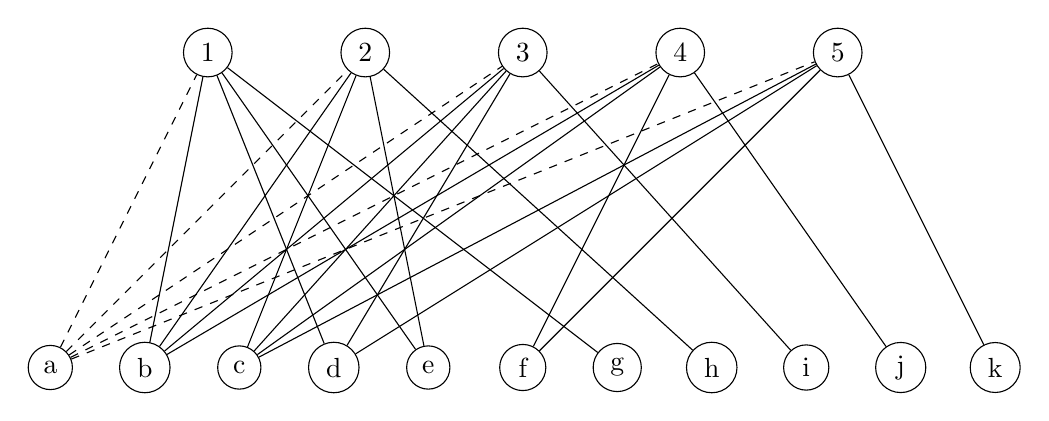
\begin{tikzpicture}[auto]
   \begin{scope}[every node/.style={circle,draw=black}]
    \node (l1) at (-4,1) {1};
    \node (l2) at (-2,1) {2};
    \node (l3) at (0,1) {3};
    \node (l4) at (2,1) {4};
    \node (l5) at (4,1) {5};
    \node (r1) at (-6,-3) {a};
    \node (r2) at (-4.8,-3) {b};
    \node (r3) at (-3.6,-3) {c};
    \node (r4) at (-2.4,-3) {d};
    \node (r5) at (-1.2,-3) {e};
    \node (r6) at (0,-3) {f};
    \node (r7) at (1.2,-3) {g};
    \node (r8) at (2.4,-3) {h};
    \node (r9) at (3.6,-3) {i};
    \node (r10) at (4.8,-3) {j};
    \node (r11) at (6,-3) {k};
   \end{scope}
   \begin{scope}[every edge/.style={draw=black}]
    \draw  (r1) [dashed] edge node{ } (l1);
    \draw  (r1) [dashed] edge node{ } (l2);
    \draw  (r1) [dashed] edge node{ } (l3);
    \draw  (r1) [dashed] edge node{ } (l4);
    \draw  (r1) [dashed] edge node{ } (l5);
    \draw  (r2) edge node{ } (l1);
    \draw  (r2) edge node{ } (l2);
    \draw  (r2) edge node{ } (l3);
    \draw  (r2) edge node{ } (l4);
    \draw  (r3) edge node{ } (l2);
    \draw  (r3) edge node{ } (l3);
    \draw  (r3) edge node{ } (l4);
    \draw  (r3) edge node{ } (l5);
    \draw  (r4) edge node{ } (l1);
    \draw  (r4) edge node{ } (l3);
    \draw  (r4) edge node{ } (l5);
    \draw  (r5) edge node{ } (l1);
    \draw  (r5) edge node{ } (l2);
    \draw  (r6) edge node{ } (l4);
    \draw  (r6) edge node{ } (l5);
    \draw  (r7) edge node{ } (l1);
    \draw  (r8) edge node{ } (l2);
    \draw  (r9) edge node{ } (l3);
    \draw  (r10) edge node{ } (l4);
    \draw  (r11) edge node{ } (l5);
   \end{scope}
\end{tikzpicture}
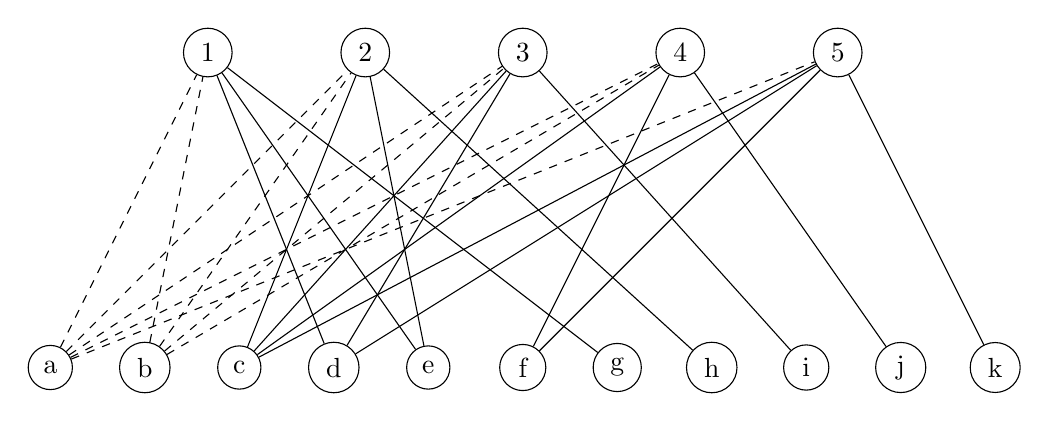
\begin{tikzpicture}[auto]
   \begin{scope}[every node/.style={circle,draw=black}]
    \node (l1) at (-4,1) {1};
    \node (l2) at (-2,1) {2};
    \node (l3) at (0,1) {3};
    \node (l4) at (2,1) {4};
    \node (l5) at (4,1) {5};
    \node (r1) at (-6,-3) {a};
    \node (r2) at (-4.8,-3) {b};
    \node (r3) at (-3.6,-3) {c};
    \node (r4) at (-2.4,-3) {d};
    \node (r5) at (-1.2,-3) {e};
    \node (r6) at (0,-3) {f};
    \node (r7) at (1.2,-3) {g};
    \node (r8) at (2.4,-3) {h};
    \node (r9) at (3.6,-3) {i};
    \node (r10) at (4.8,-3) {j};
    \node (r11) at (6,-3) {k};
   \end{scope}
   \begin{scope}[every edge/.style={draw=black}]
    \draw  (r1) [dashed] edge node{ } (l1);
    \draw  (r1) [dashed] edge node{ } (l2);
    \draw  (r1) [dashed] edge node{ } (l3);
    \draw  (r1) [dashed] edge node{ } (l4);
    \draw  (r1) [dashed] edge node{ } (l5);
    \draw  (r2) [dashed] edge node{ } (l1);
    \draw  (r2) [dashed] edge node{ } (l2);
    \draw  (r2) [dashed] edge node{ } (l3);
    \draw  (r2) [dashed] edge node{ } (l4);
    \draw  (r3) edge node{ } (l2);
    \draw  (r3) edge node{ } (l3);
    \draw  (r3) edge node{ } (l4);
    \draw  (r3) edge node{ } (l5);
    \draw  (r4) edge node{ } (l1);
    \draw  (r4) edge node{ } (l3);
    \draw  (r4) edge node{ } (l5);
    \draw  (r5) edge node{ } (l1);
    \draw  (r5) edge node{ } (l2);
    \draw  (r6) edge node{ } (l4);
    \draw  (r6) edge node{ } (l5);
    \draw  (r7) edge node{ } (l1);
    \draw  (r8) edge node{ } (l2);
    \draw  (r9) edge node{ } (l3);
    \draw  (r10) edge node{ } (l4);
    \draw  (r11) edge node{ } (l5);
   \end{scope}
\end{tikzpicture}
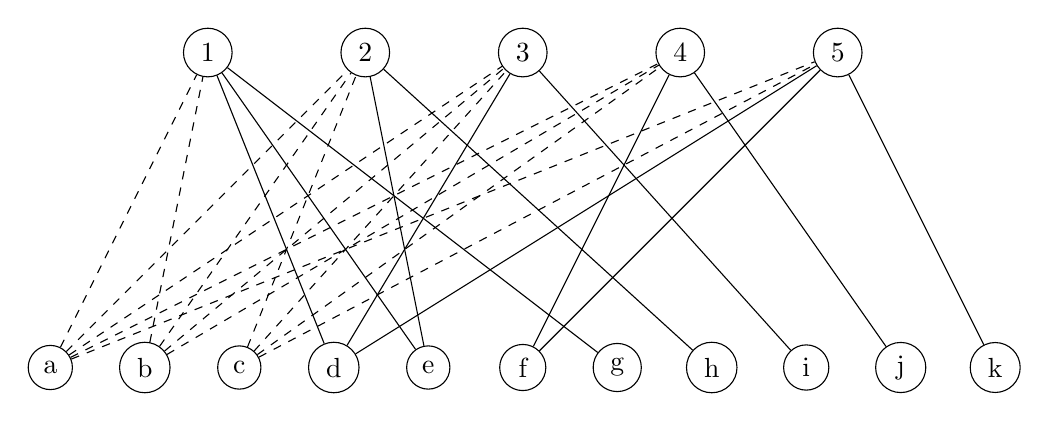
\begin{tikzpicture}[auto]
   \begin{scope}[every node/.style={circle,draw=black}]
    \node (l1) at (-4,1) {1};
    \node (l2) at (-2,1) {2};
    \node (l3) at (0,1) {3};
    \node (l4) at (2,1) {4};
    \node (l5) at (4,1) {5};
    \node (r1) at (-6,-3) {a};
    \node (r2) at (-4.8,-3) {b};
    \node (r3) at (-3.6,-3) {c};
    \node (r4) at (-2.4,-3) {d};
    \node (r5) at (-1.2,-3) {e};
    \node (r6) at (0,-3) {f};
    \node (r7) at (1.2,-3) {g};
    \node (r8) at (2.4,-3) {h};
    \node (r9) at (3.6,-3) {i};
    \node (r10) at (4.8,-3) {j};
    \node (r11) at (6,-3) {k};
   \end{scope}
   \begin{scope}[every edge/.style={draw=black}]
    \draw  (r1) [dashed] edge node{ } (l1);
    \draw  (r1) [dashed] edge node{ } (l2);
    \draw  (r1) [dashed] edge node{ } (l3);
    \draw  (r1) [dashed] edge node{ } (l4);
    \draw  (r1) [dashed] edge node{ } (l5);
    \draw  (r2) [dashed] edge node{ } (l1);
    \draw  (r2) [dashed] edge node{ } (l2);
    \draw  (r2) [dashed] edge node{ } (l3);
    \draw  (r2) [dashed] edge node{ } (l4);
    \draw  (r3) [dashed] edge node{ } (l2);
    \draw  (r3) [dashed] edge node{ } (l3);
    \draw  (r3) [dashed] edge node{ } (l4);
    \draw  (r3) [dashed] edge node{ } (l5);
    \draw  (r4) edge node{ } (l1);
    \draw  (r4) edge node{ } (l3);
    \draw  (r4) edge node{ } (l5);
    \draw  (r5) edge node{ } (l1);
    \draw  (r5) edge node{ } (l2);
    \draw  (r6) edge node{ } (l4);
    \draw  (r6) edge node{ } (l5);
    \draw  (r7) edge node{ } (l1);
    \draw  (r8) edge node{ } (l2);
    \draw  (r9) edge node{ } (l3);
    \draw  (r10) edge node{ } (l4);
    \draw  (r11) edge node{ } (l5);
   \end{scope}
\end{tikzpicture}
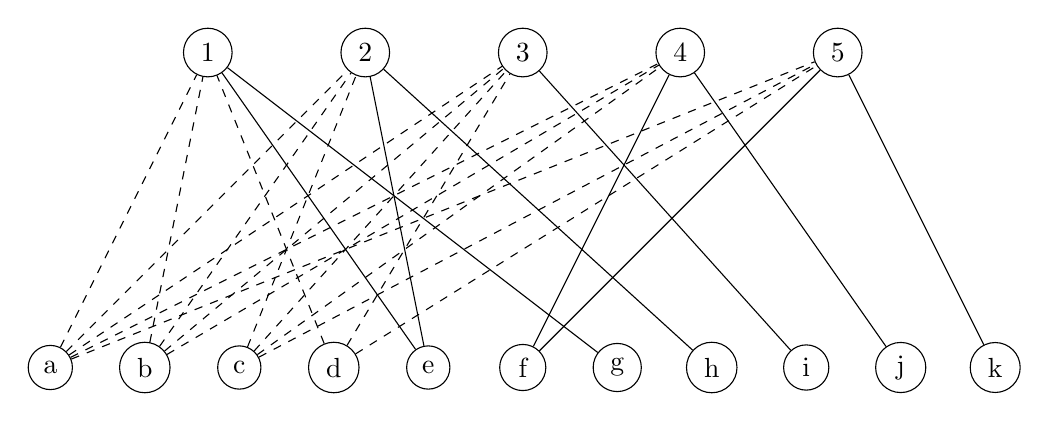
\begin{tikzpicture}[auto]
   \begin{scope}[every node/.style={circle,draw=black}]
    \node (l1) at (-4,1) {1};
    \node (l2) at (-2,1) {2};
    \node (l3) at (0,1) {3};
    \node (l4) at (2,1) {4};
    \node (l5) at (4,1) {5};
    \node (r1) at (-6,-3) {a};
    \node (r2) at (-4.8,-3) {b};
    \node (r3) at (-3.6,-3) {c};
    \node (r4) at (-2.4,-3) {d};
    \node (r5) at (-1.2,-3) {e};
    \node (r6) at (0,-3) {f};
    \node (r7) at (1.2,-3) {g};
    \node (r8) at (2.4,-3) {h};
    \node (r9) at (3.6,-3) {i};
    \node (r10) at (4.8,-3) {j};
    \node (r11) at (6,-3) {k};
   \end{scope}
   \begin{scope}[every edge/.style={draw=black}]
    \draw  (r1) [dashed] edge node{ } (l1);
    \draw  (r1) [dashed] edge node{ } (l2);
    \draw  (r1) [dashed] edge node{ } (l3);
    \draw  (r1) [dashed] edge node{ } (l4);
    \draw  (r1) [dashed] edge node{ } (l5);
    \draw  (r2) [dashed] edge node{ } (l1);
    \draw  (r2) [dashed] edge node{ } (l2);
    \draw  (r2) [dashed] edge node{ } (l3);
    \draw  (r2) [dashed] edge node{ } (l4);
    \draw  (r3) [dashed] edge node{ } (l2);
    \draw  (r3) [dashed] edge node{ } (l3);
    \draw  (r3) [dashed] edge node{ } (l4);
    \draw  (r3) [dashed] edge node{ } (l5);
    \draw  (r4) [dashed] edge node{ } (l1);
    \draw  (r4) [dashed] edge node{ } (l3);
    \draw  (r4) [dashed] edge node{ } (l5);
    \draw  (r5) edge node{ } (l1);
    \draw  (r5) edge node{ } (l2);
    \draw  (r6) edge node{ } (l4);
    \draw  (r6) edge node{ } (l5);
    \draw  (r7) edge node{ } (l1);
    \draw  (r8) edge node{ } (l2);
    \draw  (r9) edge node{ } (l3);
    \draw  (r10) edge node{ } (l4);
    \draw  (r11) edge node{ } (l5);
   \end{scope}
\end{tikzpicture}
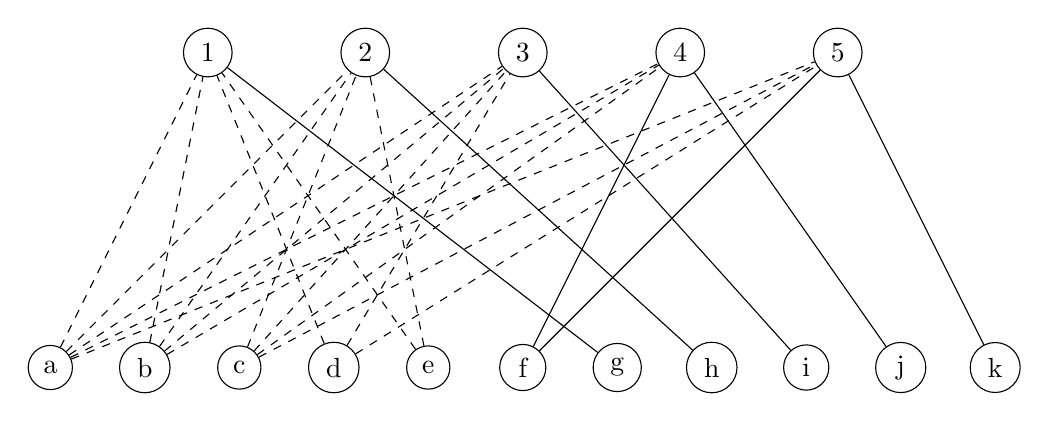
\begin{tikzpicture}[auto]
   \begin{scope}[every node/.style={circle,draw=black}]
    \node (l1) at (-4,1) {1};
    \node (l2) at (-2,1) {2};
    \node (l3) at (0,1) {3};
    \node (l4) at (2,1) {4};
    \node (l5) at (4,1) {5};
    \node (r1) at (-6,-3) {a};
    \node (r2) at (-4.8,-3) {b};
    \node (r3) at (-3.6,-3) {c};
    \node (r4) at (-2.4,-3) {d};
    \node (r5) at (-1.2,-3) {e};
    \node (r6) at (0,-3) {f};
    \node (r7) at (1.2,-3) {g};
    \node (r8) at (2.4,-3) {h};
    \node (r9) at (3.6,-3) {i};
    \node (r10) at (4.8,-3) {j};
    \node (r11) at (6,-3) {k};
   \end{scope}
   \begin{scope}[every edge/.style={draw=black}]
    \draw  (r1) [dashed] edge node{ } (l1);
    \draw  (r1) [dashed] edge node{ } (l2);
    \draw  (r1) [dashed] edge node{ } (l3);
    \draw  (r1) [dashed] edge node{ } (l4);
    \draw  (r1) [dashed] edge node{ } (l5);
    \draw  (r2) [dashed] edge node{ } (l1);
    \draw  (r2) [dashed] edge node{ } (l2);
    \draw  (r2) [dashed] edge node{ } (l3);
    \draw  (r2) [dashed] edge node{ } (l4);
    \draw  (r3) [dashed] edge node{ } (l2);
    \draw  (r3) [dashed] edge node{ } (l3);
    \draw  (r3) [dashed] edge node{ } (l4);
    \draw  (r3) [dashed] edge node{ } (l5);
    \draw  (r4) [dashed] edge node{ } (l1);
    \draw  (r4) [dashed] edge node{ } (l3);
    \draw  (r4) [dashed] edge node{ } (l5);
    \draw  (r5) [dashed] edge node{ } (l1);
    \draw  (r5) [dashed] edge node{ } (l2);
    \draw  (r6) edge node{ } (l4);
    \draw  (r6) edge node{ } (l5);
    \draw  (r7) edge node{ } (l1);
    \draw  (r8) edge node{ } (l2);
    \draw  (r9) edge node{ } (l3);
    \draw  (r10) edge node{ } (l4);
    \draw  (r11) edge node{ } (l5);
   \end{scope}
\end{tikzpicture}
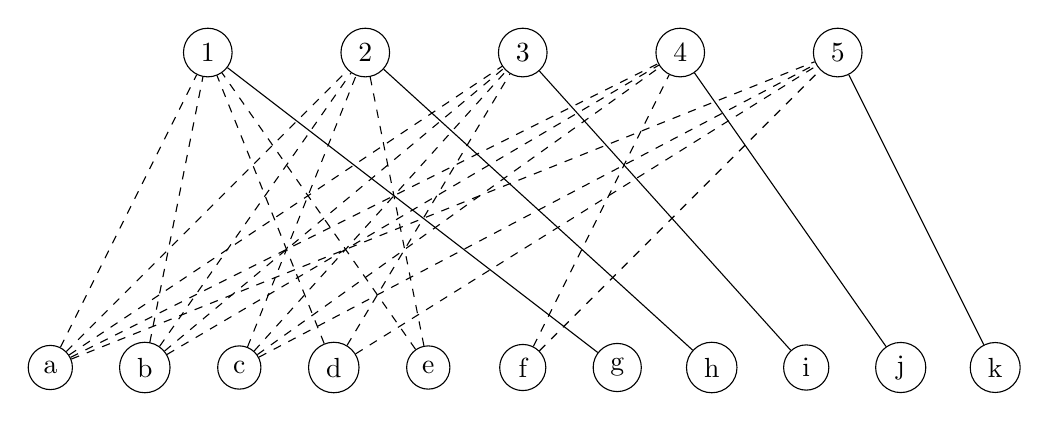
\begin{tikzpicture}[auto]
   \begin{scope}[every node/.style={circle,draw=black}]
    \node (l1) at (-4,1) {1};
    \node (l2) at (-2,1) {2};
    \node (l3) at (0,1) {3};
    \node (l4) at (2,1) {4};
    \node (l5) at (4,1) {5};
    \node (r1) at (-6,-3) {a};
    \node (r2) at (-4.8,-3) {b};
    \node (r3) at (-3.6,-3) {c};
    \node (r4) at (-2.4,-3) {d};
    \node (r5) at (-1.2,-3) {e};
    \node (r6) at (0,-3) {f};
    \node (r7) at (1.2,-3) {g};
    \node (r8) at (2.4,-3) {h};
    \node (r9) at (3.6,-3) {i};
    \node (r10) at (4.8,-3) {j};
    \node (r11) at (6,-3) {k};
   \end{scope}
   \begin{scope}[every edge/.style={draw=black}]
    \draw  (r1) [dashed] edge node{ } (l1);
    \draw  (r1) [dashed] edge node{ } (l2);
    \draw  (r1) [dashed] edge node{ } (l3);
    \draw  (r1) [dashed] edge node{ } (l4);
    \draw  (r1) [dashed] edge node{ } (l5);
    \draw  (r2) [dashed] edge node{ } (l1);
    \draw  (r2) [dashed] edge node{ } (l2);
    \draw  (r2) [dashed] edge node{ } (l3);
    \draw  (r2) [dashed] edge node{ } (l4);
    \draw  (r3) [dashed] edge node{ } (l2);
    \draw  (r3) [dashed] edge node{ } (l3);
    \draw  (r3) [dashed] edge node{ } (l4);
    \draw  (r3) [dashed] edge node{ } (l5);
    \draw  (r4) [dashed] edge node{ } (l1);
    \draw  (r4) [dashed] edge node{ } (l3);
    \draw  (r4) [dashed] edge node{ } (l5);
    \draw  (r5) [dashed] edge node{ } (l1);
    \draw  (r5) [dashed] edge node{ } (l2);
    \draw  (r6) [dashed] edge node{ } (l4);
    \draw  (r6) [dashed] edge node{ } (l5);
    \draw  (r7) edge node{ } (l1);
    \draw  (r8) edge node{ } (l2);
    \draw  (r9) edge node{ } (l3);
    \draw  (r10) edge node{ } (l4);
    \draw  (r11) edge node{ } (l5);
   \end{scope}
\end{tikzpicture}
\end{center}
We can get a vertex cover \{a,b,c,d,e,f,g,h,i,j,k\}, thus the approximation ratio is $11/5>2$.
\end{document}

